\section{Core Language}	

Zombie works on a purely functional language with products, sum types,
and first-class functions called $\lambda_Z$. For simplicity in this
paper, we treat the language as untyped. The syntax of $\lambda_Z$ is
shown in \Cref{fig:syntax}; its semantics are standard. The full
Zombie implementation supports additional features, such as primitive
types and input/output; \Cref{sec:impl} describes how these features
are layered on top of the core implementation described here.

Importantly, because Zombie is purely functional, programs are totally
deterministic, in the sense that evaluating a given expression in a
given environment always returns the same result. This is essential
for Zombie to work correctly.

\subsection{CEK Machine}

The key insight of Zombie is to assign an unique identifier to any
value ever allocated during the program's execution. Conceptually, it
identifies each value with the execution step that allocated it. It
does this using a variant of the CEK machine.

The CEK machine is a well-known abstract machine for executing untyped
lambda calculi, where the machine state consists of three parts:

\begin{enumerate}
	\item \textcolor{blue}{C}ontrol, the expression currently being evaluated.
	\item \textcolor{blue}{E}nvironment,
          a map from the free variables of the Control to their values.
	\item \textcolor{blue}{K}ontinuation, which is to be invoked
          with the value the Control evaluates to.
\end{enumerate}

In our variation of the CEK machine, we split the evaluation phase
from the invocation of the continuation, resulting in a machine state
that looks like this:
\[
\text{State} \operatorname{::=} \Eval~C~\Env~K \mid \Apply~K~V
\]
In other words, our CEK machine can be in an $\Eval$ or an $\Apply$
state; the $\Eval$ stores the classic control, environment, and
kontinuation, while the $\Apply$ state stores just a continuation and
a value. The precise syntax of values and kontinuations are given in
\Cref{fig:defs}.

Execution in the CEK machine involves a series of transitions between
these machine states; in other words, it is a transition system. To
run a program $C$ in the CEK machine, one first sets up an initial
state $(\Eval~C~\{\}~\Done)$ whose Control is the expression to
evaluate, whose Environment is empty, and whose Kontinuation is a
special $\Done$ continuation. The rules of the CEK machine are then
used to transition from one machine state to another, until finally
reaching the state $\Apply~\Done~V$. In that state, $V$ is the result
of evaluating of $C$.%
\footnote{Note that, because $\lambda_Z$ is untyped, it contains
non-terminating programs using, for example, the $Y$ combinator. In
the CEK machine, these programs create an infinite sequence of machine
states that do not include a terminating $\Apply~\Done~V$.}

A notable property of the CEK machine is that each transition performs
a bounded amount of work. Contrast this to a traditional operation
semantics, where the semantics of a \sCase statement might be something
like:

\begin{mathpar}
 \inferrule{
   \Gamma \vdash e \to^* \sLeft~\Gamma' \vdash V
 }{\Gamma \vdash \sCase~e~x~e_l~y~e_r
   \to \Gamma', x : V \vdash e_l
 }
\end{mathpar}

Here the antecedent of the inference rule might perform arbitrarily
many steps, and thus an arbitrary amount of computation; derivations
thus form a tree. In the CEK machine, no such steps exist, and
derivations in the CEK machine form a flat list. This property of the
CEK machine is illustrated graphically in \Cref{fig:constant}.

\begin{figure}
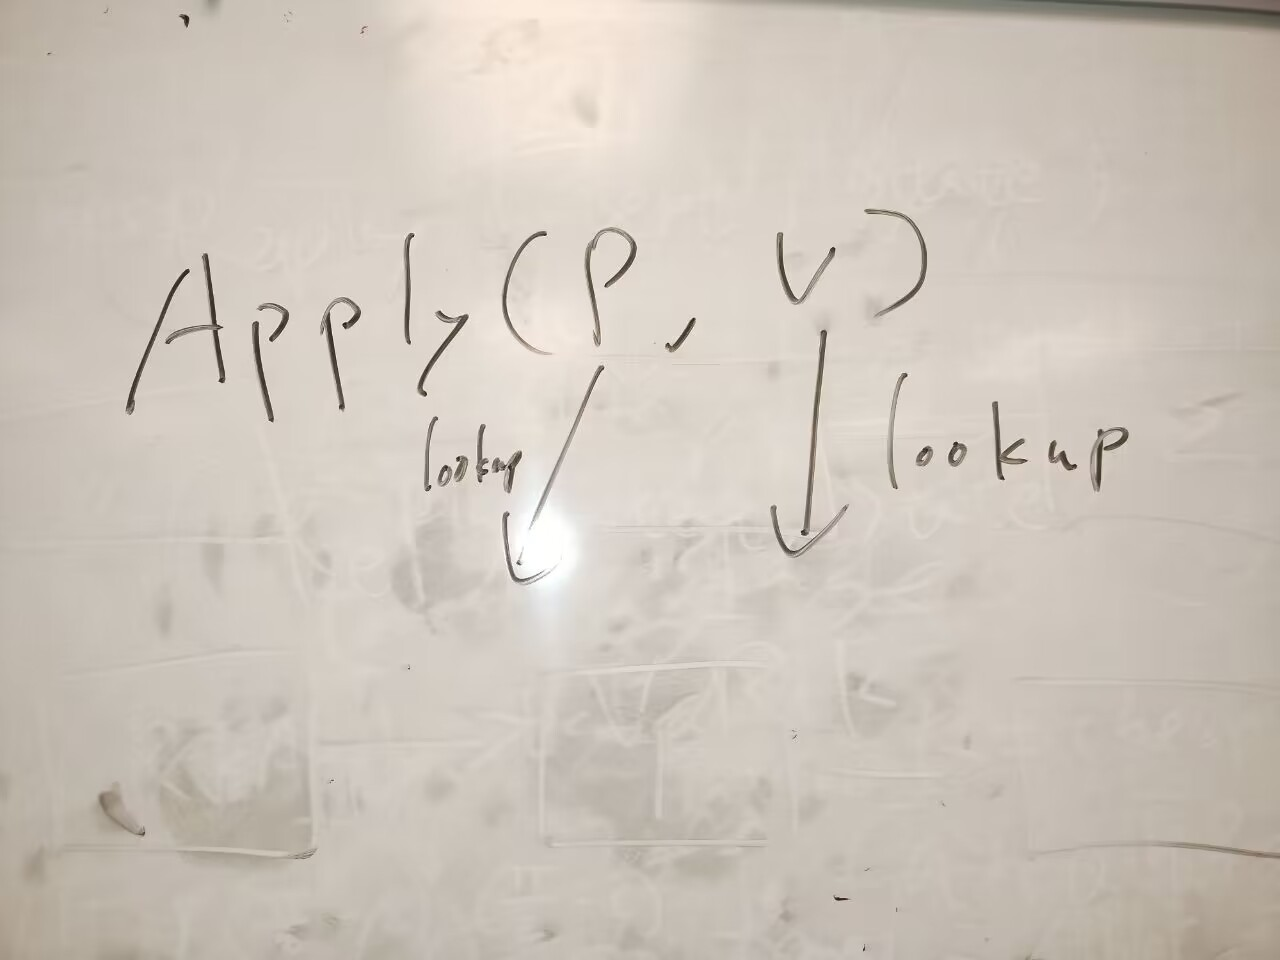
\includegraphics[width=0.5\columnwidth]{1}
\caption{the machine does a small constant amount of pointer lookup}
\label{fig:constant}
\end{figure}

\subsection{Determinism and Tocks}

Importantly, the CEK machine is linear and deterministic. This means
that every CEK machine state transitions to at most one state. That in
turn means that if we were to ``rewind'' a CEK machine, putting it in
an earlier state, it would transition through the exact same sequence
of states in the exact same order. This determinism or
``replayability'' is essential for Zombie to work, and is illustrated
graphically in \Cref{fig:replayability}.

\begin{figure}
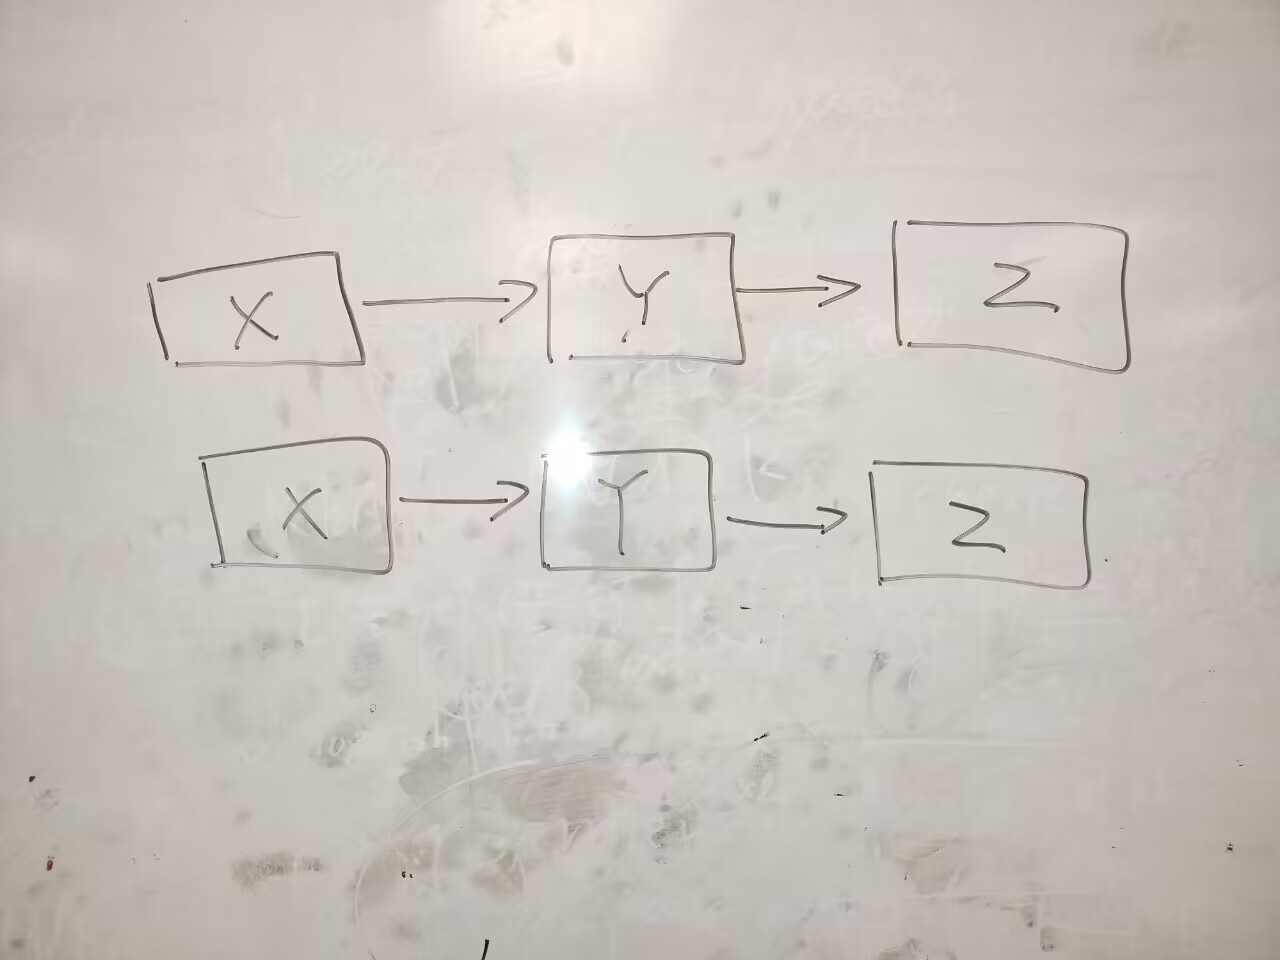
\includegraphics[width=0.5\columnwidth]{0}
\caption{the deterministic, linear nature of the CEK machine}
\label{fig:replayability}
\end{figure}

One key property guaranteed by determinism is that, for a given
initial program $C$, the machine state at any point during $C$'s
execution can be uniquely identified by how many steps have been
executed since the initial state. In other words, the initial state is
identified with the number $0$, the next state it transitions to with
the number $1$, and so on. This state number, which we call a
``tock'', is logically unbounded, but in our implementation it is
stored as a 64-bit integer. In our implementation, that suffices for
several decades of runtime on current hardware. 

\subsection{Heap Memory}

Because we are interested the total memory usage of $\lambda_Z$
program, our variant of the CEK machine includes an explicit heap and
explicit pointers. That is, in our formalization values $V$ are
formalized as pointers $P\langle \VCell \rangle$ to ``value cells''.
Values cells---which can be closures, products, and sums---in turn
contain values, that is, pointers.

During execution, the CEK machine looks up these values using an
explicit heap $H$. To interact with the heap, the CEK machine uses two
functions. $\Lookup : (P \langle X \rangle, H) \to X$ dereferences a
pointer in the heap. $\Alloc : (X, H) \to (P \langle X \rangle, H')$
stores a value in the heap, returning a pointer to it and the updated
heap. Transitions in the CEK machine call $\Lookup$ and $\Alloc$ in
order to make $\Eval$ and $\Apply$ steps, as shown in \Cref{fig:eval}
and \Cref{fig:apply}.

Importantly, every CEK machine step (whether $\Eval$ or $\Apply$)
makes at most one call to $\Lookup$ and at most one call to $\Alloc$. 
This means that each allocation the program
makes can be uniquely identified by the tock for the machine state
where it is allocated. This identification is the core abstraction
that drives Zombie's implementation.

\newcommand{\mytableshape}{p{6em} p{2.6em} p{1em} p{0.45\textwidth}}
\begin{figure}
	\begin{tabular}{\mytableshape}
		Name & $N$ & $::=$ & A set of distinct names \\
		Expr & $C$ & $::=$ & $
		N \mid
		\sLet~x=A~\sIn~B \mid
		\backslash x.~A \mid
		f(x) \mid
		(x, y) \mid
		x.0 \mid
		x.1 \mid
		\sLeft~x \mid
		\sRight~y \mid
		\sCase~x~\sOf~\sLeft~a\Rightarrow L~||~\sRight~b\Rightarrow R $
	\end{tabular}
	\caption{The syntax of $\lambda_Z$.}
        \label{fig:syntax}
\end{figure}

\begin{figure}
	\begin{tabular}{\mytableshape}
		Heap & $H$ & $::=$ & An abstract key value store \\
		Pointer$\langle X \rangle$ & $P\langle X \rangle$ & $::=$ & Key into heap with value type $X$ \\
		Lookup & & : & $(\text{Pointer}\langle X \rangle, H) \to X$ \\
		Alloc & & : & $(X, H) \to (\text{Pointer}\langle X \rangle, H)$ \\
	\end{tabular}
	\caption{Heap API}
	\label{fig:heap}
\end{figure}

\begin{figure}
	\begin{tabular}{\mytableshape}
		Continuation & $K$ & $::=$ & $P \langle \KCell \rangle$ \\
		
		KCell & & $::=$ & $
		\Done \mid
		KLookup~K~ \mid
		\KLet~N~\Env~C~K \mid
		\KApp_0~\Env~C~K \mid
		\KApp_1~\Env~N~C~K \mid
		\KProd_0~\Env~C~K \mid
		\KProd_1~V~K \mid
		\KZro~K \mid
		\KFst~K \mid
		\KLeft~K \mid
		\KRight~K \mid
		\KCase~\Env~N~C~N~C~K $ \\
		
		Value & $V$ & $::=$ & $P\langle \VCell \rangle$ \\
		VCell & & $::=$ & $
		\Clos~\Env~N~E \mid
		\VProd~V~V \mid
		\VLeft~V \mid
		\VRight~V $ \\
		
		Environment & $\Env$ & ::= & $[(N, V)]$ \\
		State & & ::= & $\Eval~E~\Env~K \mid \Apply~KCell~V $ \\
	\end{tabular}
	\caption{Definitions for the CEK Machine}
        \label{fig:defs}
\end{figure}
\begin{figure}
	\begin{mathpar}
		\inferrule{ }{\text{State} \leadsto \text{State}} \and
		\inferrule{ }{\Eval(N, \Env, K) \leadsto \Apply(K, \Env(N))} \and
		\inferrule{ }{\Eval(\sLet~A=B~\sIn~C, \Env, K) \leadsto \Eval(B, \Env, \KLet~A~K~C~\Env)} \and
		\inferrule{ }{\Apply(\KLet~A~\Env~C~K, V) \leadsto \Eval(C, \Env[A := V], K)} \and
		\inferrule{ }{\Eval(\backslash N. C, \Env, K) \leadsto \Apply(K, \Clos~\Env(\text{fv})\cdots N~C)} \and
		\inferrule{ }{\Eval(F(X), \Env, K) \leadsto \Eval(F, \KApp_0~K~X)} \and
		\inferrule{ }{\Apply(\KApp_0~\Env~X~K, \Clos~\Env'~N~C) \leadsto \Eval(X, \Env, \KApp_1~\Env'~N~C~K)} \and
		\inferrule{ }{\Apply(\KApp_1~\Env~N~C~K, V) \leadsto \Eval(C, \Env[N := V], K)}
		\inferrule{ }{\Eval((L, R), \Env, K) \leadsto \Eval(L, \Env, \KProd_0~K~R)} \and
		\inferrule{ }{\Apply(\text{KProd0}~\Env~R~K, V) \leadsto \Eval(R, Env, \KProd_1~V~K)} \and
		\inferrule{ }{\Apply(\KProd_1~L~K, V) \leadsto \Apply(K, \VProd~L~V)} \and
		\inferrule{ }{\Eval(X.0, \Env, K) \leadsto \Eval(X, \Env, \KZro~K)} \and
		\inferrule{ }{\Apply(\KZro~K, \VProd~X~Y) \leadsto \Apply(K, X)} \and
		\inferrule{ }{\Eval(X.1, \Env, K) \leadsto \Eval(X, \Env, \KFst~K)} \and
		\inferrule{ }{\Apply(\KFst~K, \VProd~X~Y) \leadsto \Apply(K, Y)} \and
		\inferrule{ }{\Eval(\sLeft~X, \Env, K) \leadsto \Eval(X, \Env, \KLeft~K)} \and
		\inferrule{ }{\Apply(\KLeft~K, V) \leadsto \Apply(K, \VLeft~V)} \and
		\inferrule{ }{\Eval(\sRight~X, \Env, K) \leadsto \Eval(X, \Env, \KRight~K)} \and
		\inferrule{ }{\Apply(\KRight~K, V) \leadsto \Apply(K, \VRight~V)} \and
		\inferrule{ }{\Eval(\sCase~X~\sOf~\sLeft~LN\Rightarrow L~||~\sRight~RN\Rightarrow R, \Env, K) \leadsto \Eval(X, \Env, \KCase~\mathit{LN}~L~\mathit{RN}~R~\Env)} \and
		\inferrule{ }{\Apply(\KCase~\Env~\mathit{LN}~L~\mathit{RN}~R~K, VLeft V) \leadsto \Eval(L, \Env[\mathit{LN} := V], K)} \and
		\inferrule{ }{\Apply(\KCase~\Env~\mathit{LN}~L~\mathit{RN}~R~K, VRight V) \leadsto \Eval(R, \Env[\mathit{RN} := V], K)} \and
	\end{mathpar}
	\caption{Abstract Machine Transition: No Pointer}
	\label{fig:apply}
\end{figure}

\begin{figure}
	\begin{mathpar}
		\inferrule{ }{\text{State}, H \leadsto \text{State}, H} \and
		\inferrule{ \Lookup(K, H) = KCell }{\Eval(N, \Env, K), H \leadsto \Apply(KCell, \Env(N)), H} \and
		\inferrule{\Alloc(\KLet~A~K~C~\Env, H) = (P, H')}{\Eval(\sLet~A=B~\sIn~C, \Env, K), H \leadsto \Eval(B, \Env, P), H'} \and
		\inferrule{ \Lookup(K, H) = KCell \and \Alloc(\Clos~\Env(\text{fv})\cdots N~C, H) = (P, H')}{\Eval(\backslash N. C, \Env, K), H \leadsto \Apply(KCell, P), H'} \and
		\inferrule{\Alloc(\KApp_0~K~X, H) = (P, H')}{\Eval(F(X), \Env, K), H \leadsto \Eval(F, P), H'} \and
		\inferrule{\Alloc(\KProd_0~K~R, H) = (P, H')}{\Eval((L, R), \Env, K), H \leadsto \Eval(L, \Env, P), H'} \and
		\inferrule{\Alloc(\KZro~K, H) = (P, H')}{\Eval(X.0, \Env, K), H \leadsto \Eval(X, \Env, P), H'} \and
		\inferrule{\Alloc(\KFst~K, H) = (P, H')}{\Eval(X.1, \Env, K), H \leadsto \Eval(X, \Env, P), H'} \and
		\inferrule{\Alloc(\KLeft~K, H) = (P, H')}{\Eval(\sLeft~X, \Env, K), H \leadsto \Eval(X, \Env, P), H'} \and
		\inferrule{\Alloc(\KRight~K, H) = (P, H')}{\Eval(\sRight~X, \Env, K), H \leadsto \Eval(X, \Env, P), H'} \and
		\inferrule{\Alloc(\KCase~\mathit{LN}~L~\mathit{RN}~R~\Env, H) = (P, H')}{\Eval(\sCase~X~\sOf~\sLeft~LN\Rightarrow L~||~\sRight~RN\Rightarrow R, \Env, K), H \leadsto \Eval(X, \Env, P), H'} \and
	\end{mathpar}
	\caption{Abstract Machine Transition: Eval}
        \label{fig:eval}
\end{figure}

\begin{figure}
	\begin{mathpar}
		\inferrule{\Lookup(K, H) = KCell}{\Apply(KLookup~ K, V), H \leadsto \Apply(KCell, V), H} \and
		\inferrule{ }{\Apply(\KLet~A~\Env~C~K, V), H \leadsto \Eval(C, \Env[A := V], K), H'} \and				\inferrule{\Lookup(V, H) = \Clos~\Env'~N~C \and \Alloc(\KApp_1~\Env'~N~C~K, H) = (P', H')}{\Apply(\KApp_0~\Env~X~K, V), H \leadsto \Eval(X, \Env, P'), H'} \and
		\inferrule{ }{\Apply(\KApp_1~\Env~N~C~K, V), H \leadsto \Eval(C, \Env[N := V], K), H'} \and
		\inferrule{\Lookup(K, H) = KCell \and \Alloc(\KProd_1~V~\Env~K, H) = (P', H')}{\Apply(\text{KProd0}~\Env~R~K, V), H \leadsto \Apply(KCell, P'), H'} \and
		\inferrule{\Lookup(K, H) = KCell \and \Alloc(\VProd~L~V, H) = (P, H')}{\Apply(\KProd_1~L~K, V), H \leadsto \Apply(KCell, P), H'} \and
		\inferrule{\Lookup(V, H) = (\VProd~X~Y)}{\Apply(\KZro~K, V), H \leadsto \Apply(KLookup~ K, X), H'} \and
		\inferrule{\Lookup(V, H) = (\VProd~X~Y)}{\Apply(\KFst~K, V), H \leadsto \Apply(KLookup~ K, Y), H'} \and
		\inferrule{\Lookup(K, H) = KCell \and \Alloc(\VLeft~V, H) = (P', H')}{\Apply(\KLeft~K, V), H \leadsto \Apply(KCell, P'), H'} \and
		\inferrule{\Lookup(K, H) = KCell \and \Alloc(\VRight~V, H) = (P', H')}{\Apply(\KRight~K, V), H \leadsto \Apply(KCell, P'), H'} \and
		\inferrule{\Lookup(V, H) = \VLeft~V'}{\Apply(\KCase~\Env~\mathit{LN}~L~\mathit{RN}~R~K, V), H \leadsto \Eval(L, \Env[\mathit{LN} := V'], K), H} \and
		\inferrule{\Lookup(V, H) = \VRight~V'}{\Apply(\KCase~\Env~\mathit{LN}~L~\mathit{RN}~R~K, V), H \leadsto \Eval(R, \Env[\mathit{RN} := V'], K), H} \and
	\end{mathpar}
	\caption{Abstract Machine Transition: Apply}
        \label{fig:apply}
\end{figure}